\section{Сколько вешать в полутонах? Интервалы}
\label{ch:harmony:interval}

\begin{Definition}[Интервал]
    \emph{Интервал} --- это расстояние между \emph{двумя} музыкальными звуками, выраженное в полутонах. 
\end{Definition}

Это определение для математиков. Для музыкантов интервалы \emph{звучат}! Если два звука прозвучали одновременно, то интервал называется \emph{гармоническим}, а если друг за другом --- \emph{мелодическим}.

\begin{Example}[Послушаем гармонические интервалы]
    \label{ex:harmony:interval:string5and6}
    Возьмите настроенную гитару. Поиграем на 5 и 6-й струне. Если гитара настроена страндартно, то 6-я струна на 5-м ладу прозвучит в унисон с открытой 5-й струной. Такое расстояние в 0 полутонов музыканты называют \emph{примой}. 
    
    Инструмент обязательно должен быть настроен! Иначе эксперимент не получится.
    
    Теперь расслабьтесь, успокойтесь, забудьте обо всех горестях и радостях. Сосредоточьтесь на своем дыхании. Существует только ваше дыхание. Абсолютный покой. 
    
    Не получается? Чёрт с ним!

    Вам нужно будет оценить свои ощущения от сыгранных интервалов. Поставьте каждому интервалу оценку, например по 5-и балльной шкале: 1(ужос), 2(срам), 3(терпимо), 4(хорошо), 5(прекрасно).
    
    Начнем. Зажимите 6-ю струну на 5-м ладу и одновременно сыграйте две струны: 6-ю и 5-ю. Звучит гармонический интервал \emph{прима}! Интервал в ноль полутонов. Прислушиваемся к ощущениям, ставим приме оценку.
    
    Продолжаем оценивать интервалы. Играем одновременно 5-ю открытую струну и 6-ю струну на 6-м ладу. Расстояние в 1 полутон. Оценивайте результат.
    
    И так далее, играем интервал в 2 полутона (6-я струна на 7-м ладу) и так далее до интервала в 12 полутонов (6-я струна на 17 ладу). 
    
    Читая этот раздел, периодически поглядывайте на свои записи. Будет полезно.
\end{Example}

Приятный на слух интервал (неважно, гармонический или мелодический) музыканты называют \emph{консонансом}, а неприятный --- \emph{диссонансом}. 

Чтобы глубже разобраться в том, почему звучание одного интервала нам нравится, а другого --- нет, визуализируем результат наложения двух звуков. Пусть функция $\sin(x)$ изображает основной тон исходного звука. Функция $\sin(x\cdot(\sqrt[12]{2})^n)$ будет изображать звук, который \emph{выше} исходного на $n$ \emph{полутонов}. Результату совместного звучания (то есть гармоническому интервалу) будет соответствовать их сумма\footnote{В Интернете масса сайтов, позволяющих построить график функции. Более того, просто вбейте в гугл \texttt{sin(x)+sin(x*(2\^{}(1/12)))} и дивитесь чудесам Технологии!}:

\begin{equation}
    \label{eq:harmony:interval:sin}
    \sin(x) + \sin(x\cdot(\sqrt[12]{2})^n).
\end{equation}

Результаты построения графиков совместного звучания (построен красным цветом) на фоне исходного звука (синий цвет) для интервалов от $n=1$ до $n=11$ полутонов (т.е. в рамках октавы) приведены в таблицах \ref{t:harmony:interval:disso-1-2-10-11}, \ref{t:harmony:interval:conso-3-4-8-9}, \ref{t:harmony:interval:conso-5-7}, \ref{t:harmony:interval:disso-6}.

Диссонансы приведены в таблицах \ref{t:harmony:interval:disso-1-2-10-11} и \ref{t:harmony:interval:disso-6}. Диссонансы получаются на интервалах в 1,2,6,10 или 11 полутонов. Значит вам не должны были понравиться интервалы на 6,7,11,15,16 ладах 6-й струны, если вы обратили внимание на пример \ref{ex:harmony:interval:string5and6}. Только не говорите, что понравились! Пора сходить к доктору!!! Не затягивайте. 

\begin{table}[!ht]
    \caption{Диссонансы в графиках функции \eqref{eq:harmony:interval:sin}}
    \label{t:harmony:interval:disso-1-2-10-11}
    \centering
    \begin{tabular}{c|c}
        \hline\hline
        1 полутон, $n=1$        & 2 полутона, $n=2$ \\
        малая секунда           & большая секунда \\
        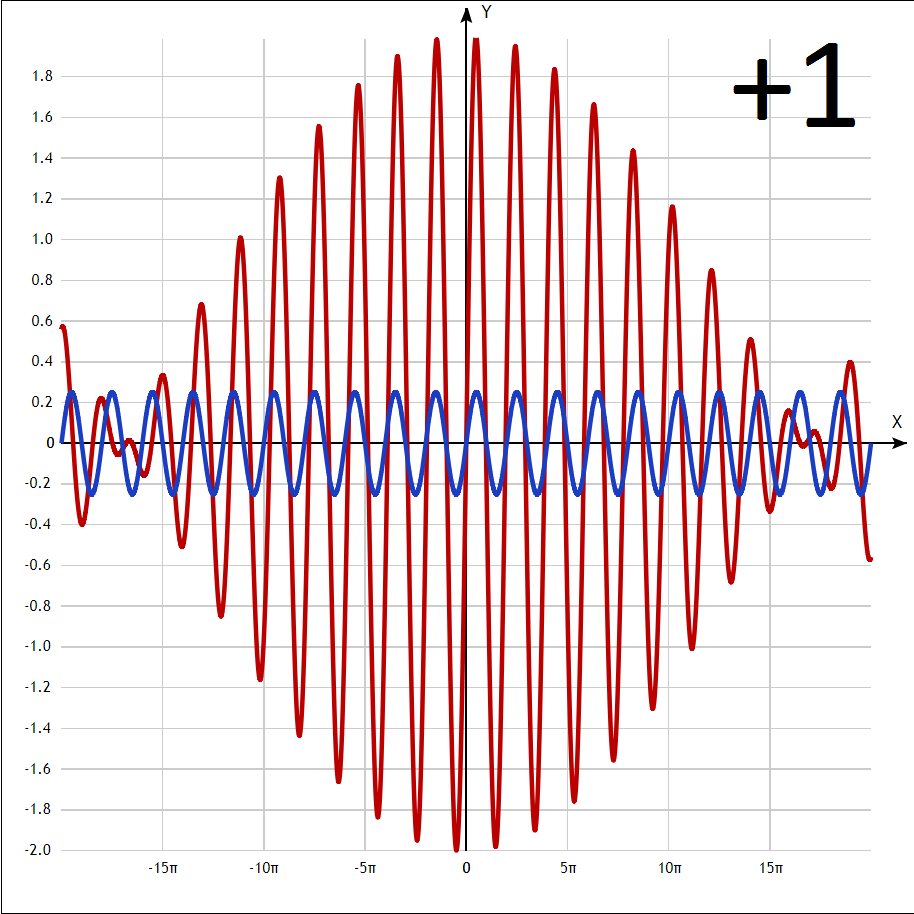
\includegraphics[width=0.45\textwidth]{fig/intervals/i01}
            & 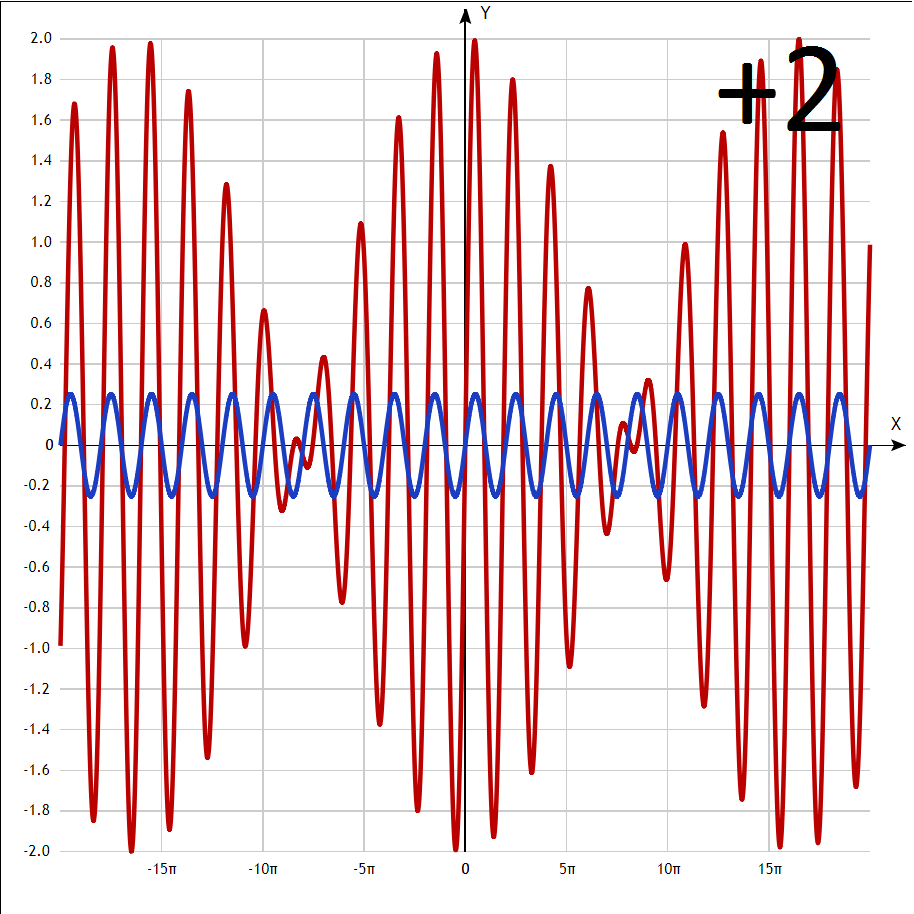
\includegraphics[width=0.45\textwidth]{fig/intervals/i02} \\
        \hline\hline
        10 полутонов, $n=10$    & 11 полутонов, $n=11$ \\
        малая септима           & большая септима \\
        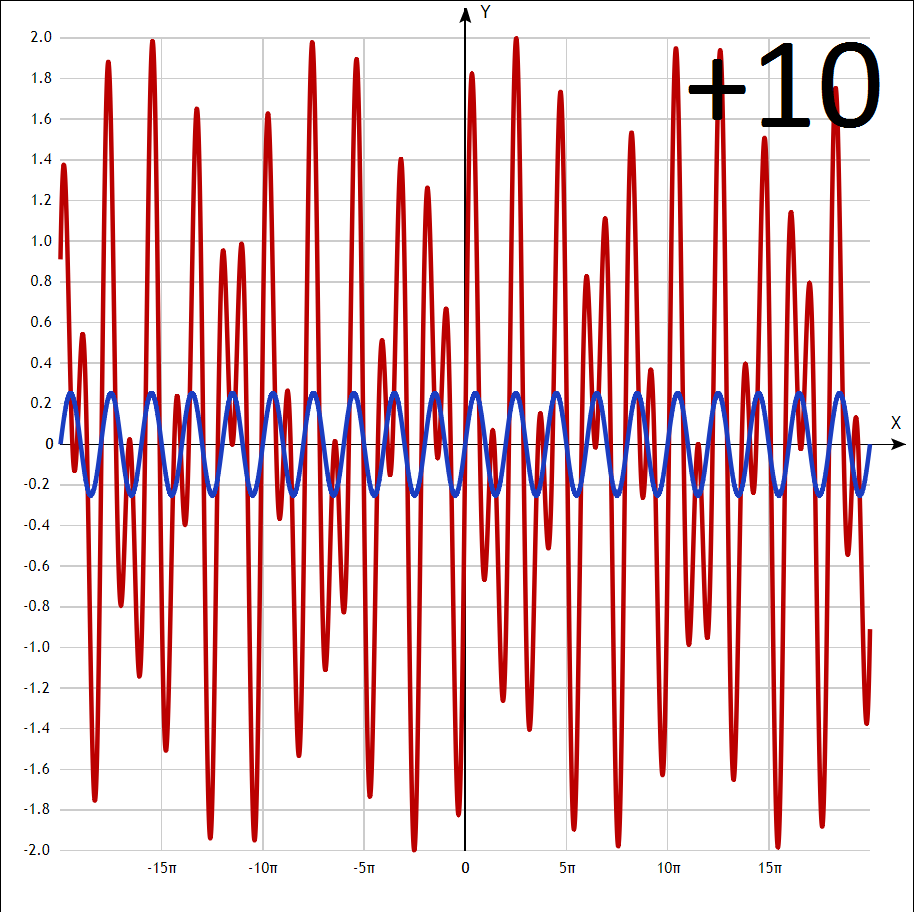
\includegraphics[width=0.45\textwidth]{fig/intervals/i10}
            & 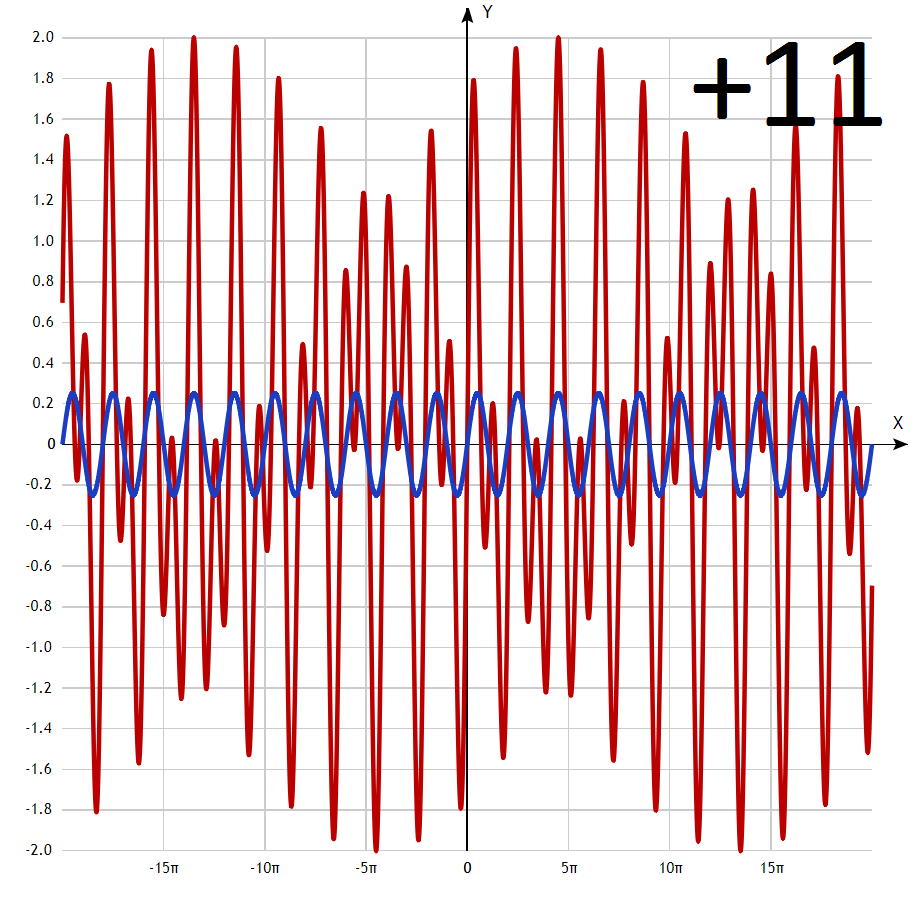
\includegraphics[width=0.45\textwidth]{fig/intervals/i11} \\
        \hline\hline
    \end{tabular}
\end{table}

Приглядитесь к приведенным графикам и попробуйте самостоятельно сделать выводы о причинах благозвучия консонансов и некоей хаотичности диссонансов. Консонансы, кстати, принято разделять на:
\begin{itemize}
    \item \emph{абсолютные}. Это полностью сливающиеся на слух интервалы в 0 полутонов (\emph{прима}, если помните) или кратные 12-ти полутонам. О причинах слияния этих звуков мы поговорили в самом начале, см. раздел \ref{ch:music:tone}. Интервал в 12 полутонов называется \emph{октавой}.
    
    \item \emph{совершенные}. Расстояние между звуками составляет 5 или 7 полутонов. См. таблицу \ref{t:harmony:interval:conso-5-7}. Смело можете понизить или повысить любой из звуков такого интервала на одну или несколько октав (12 полутонов) и совершенный консонанс останется\footnote{Уже заметили, что 5+7=12?}. Эти интервалы не сливаются на слух, но звучат благозвучно. Отличник среди консонансов.
    
    \item \emph{несовершенные}. Звуки не сливаются, точно не диссонанс, но и не совершенный консонанс. Короче, консонанс с помарочкой. Когда мы слышим несовершенный консонанс, то хочется, чтобы он побыстрее перешел консонанс совершенный, стал отличником. Разница между звуками составляет 3, 4, 8 или 9 полутонов. Точно так же, любой звук такого интервала можно понизить или повысить на октаву и несовершенство останется.
\end{itemize}


\begin{table}[!ht]
    \caption{Несовершенные консонансы в графиках функции \eqref{eq:harmony:interval:sin}}
    \label{t:harmony:interval:conso-3-4-8-9}
    \centering
    \begin{tabular}{c|c}
        \hline\hline
        3 полутона, $n=3$   & 4 полутона, $n=4$ \\
        малая терция        & большая терция \\
        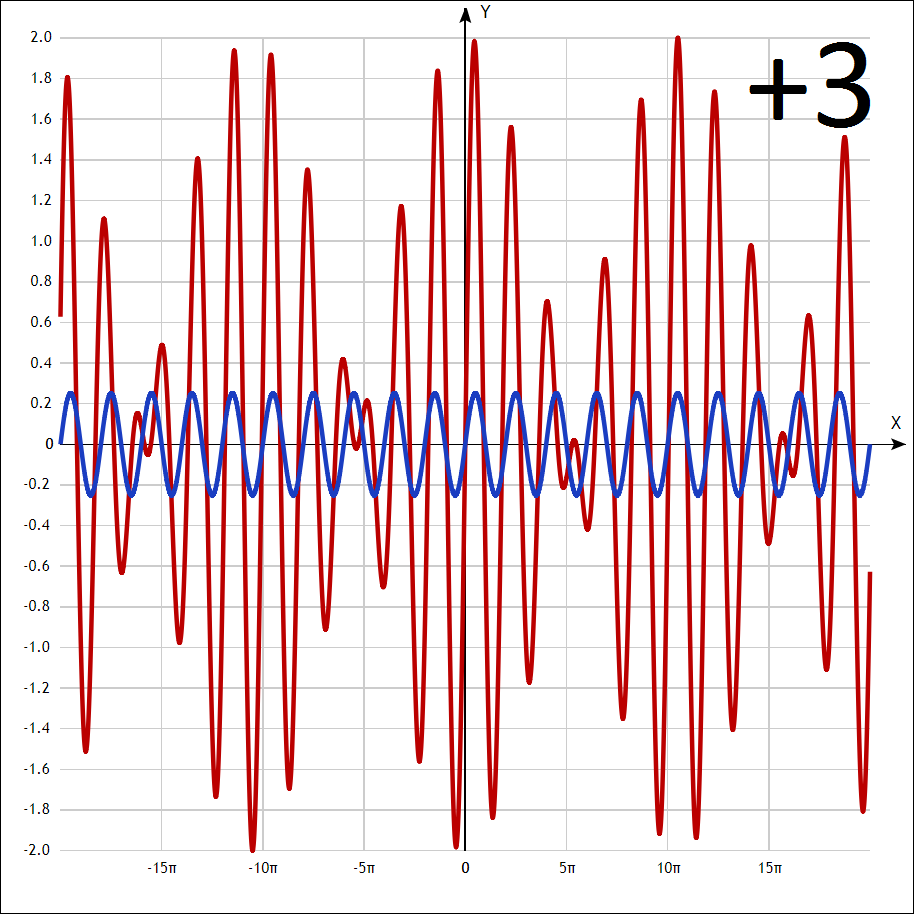
\includegraphics[width=0.45\textwidth]{fig/intervals/i03}
            & 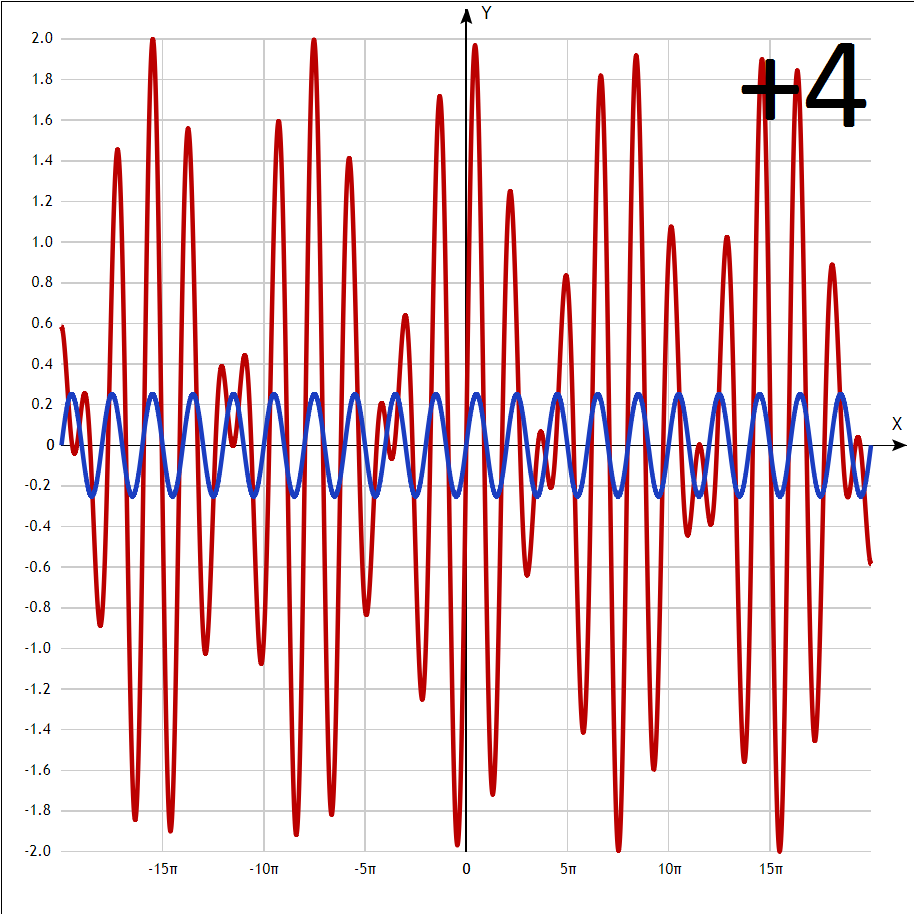
\includegraphics[width=0.45\textwidth]{fig/intervals/i04} \\
        \hline\hline
        8 полутонов, $n=8$  & 9 полутонов, $n=9$ \\
        малая секста        & большая секста \\
        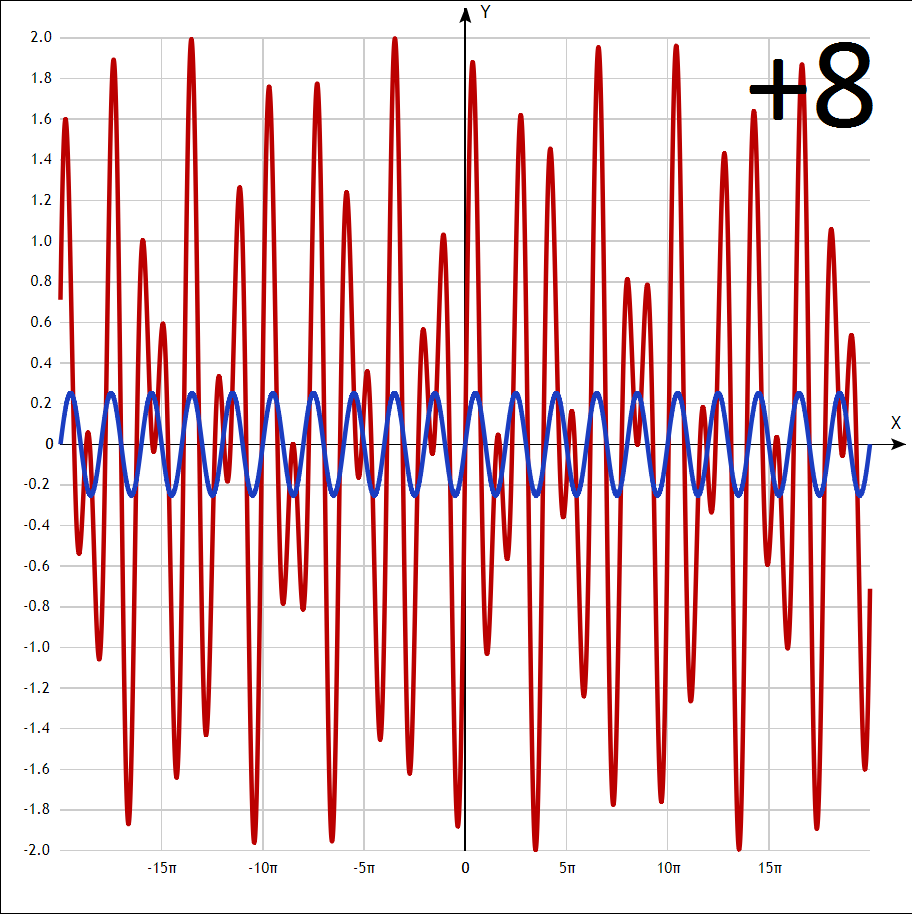
\includegraphics[width=0.45\textwidth]{fig/intervals/i08}
            & 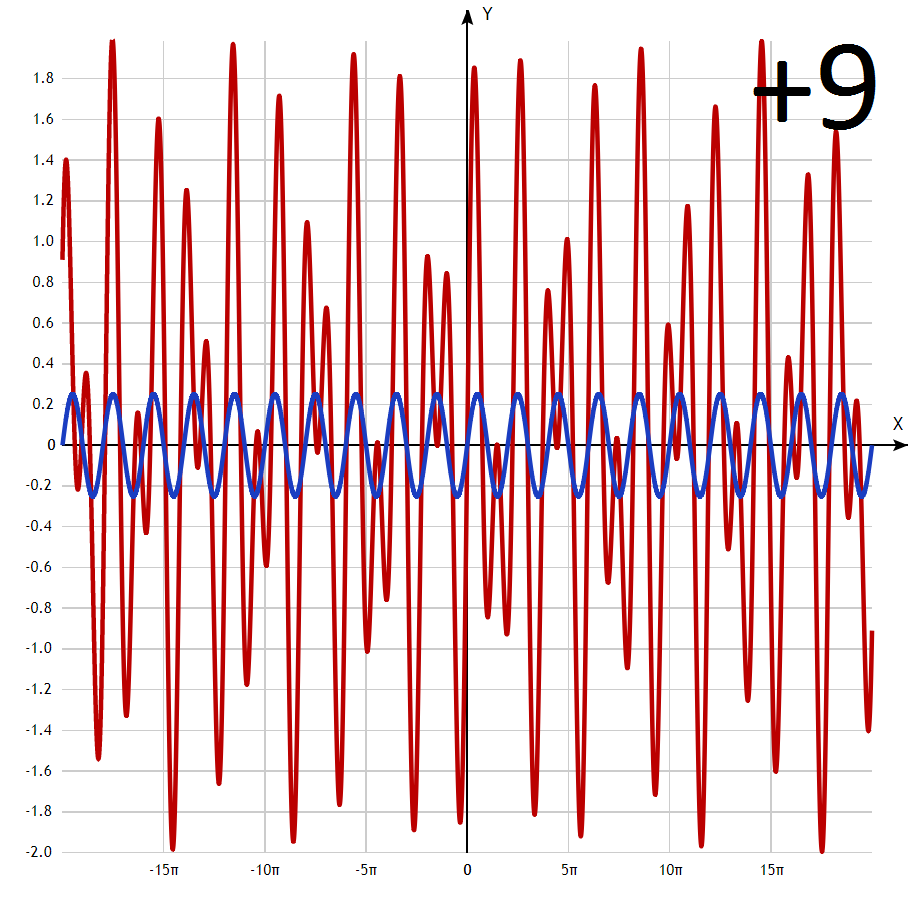
\includegraphics[width=0.45\textwidth]{fig/intervals/i09} \\
        \hline\hline
    \end{tabular}
\end{table}

\begin{table}[!ht]
    \caption{Совершенные консонансы в графиках функции \eqref{eq:harmony:interval:sin}}
    \label{t:harmony:interval:conso-5-7}
    \centering
    \begin{tabular}{c|c}
        \hline\hline
        5 полутонов, $n=5$  & 7 полутонов, $n=7$ \\
        чистая кварта       & чистая квинта \\
        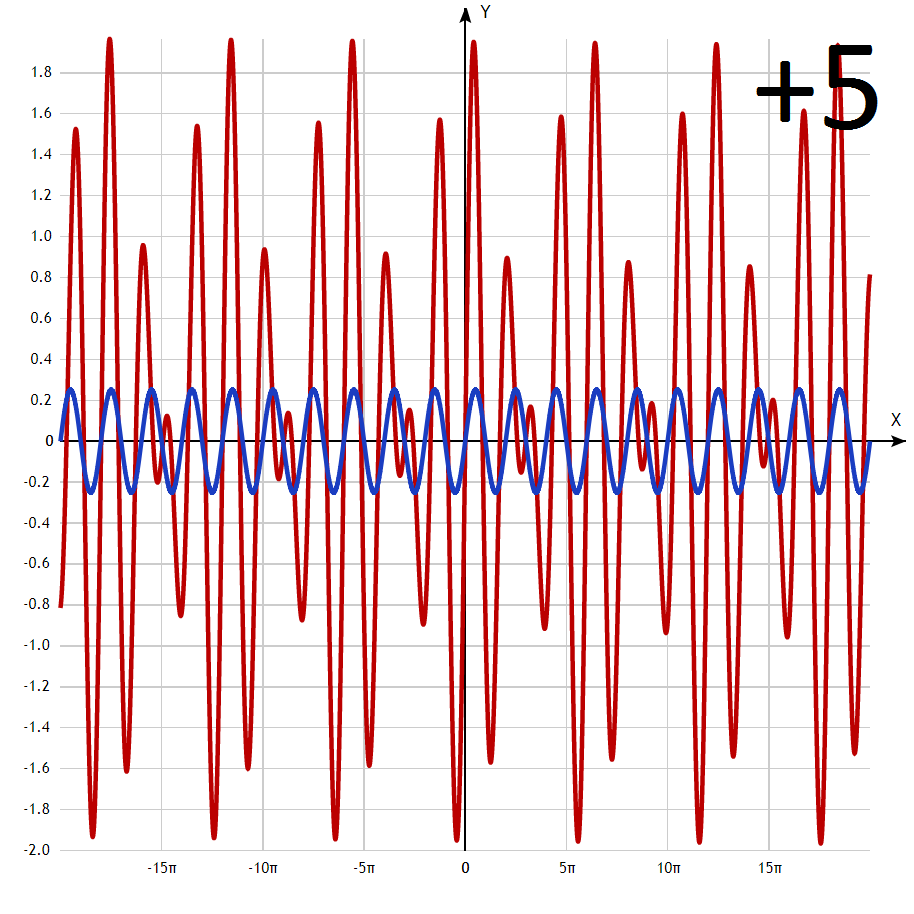
\includegraphics[width=0.45\textwidth]{fig/intervals/i05} 
            & 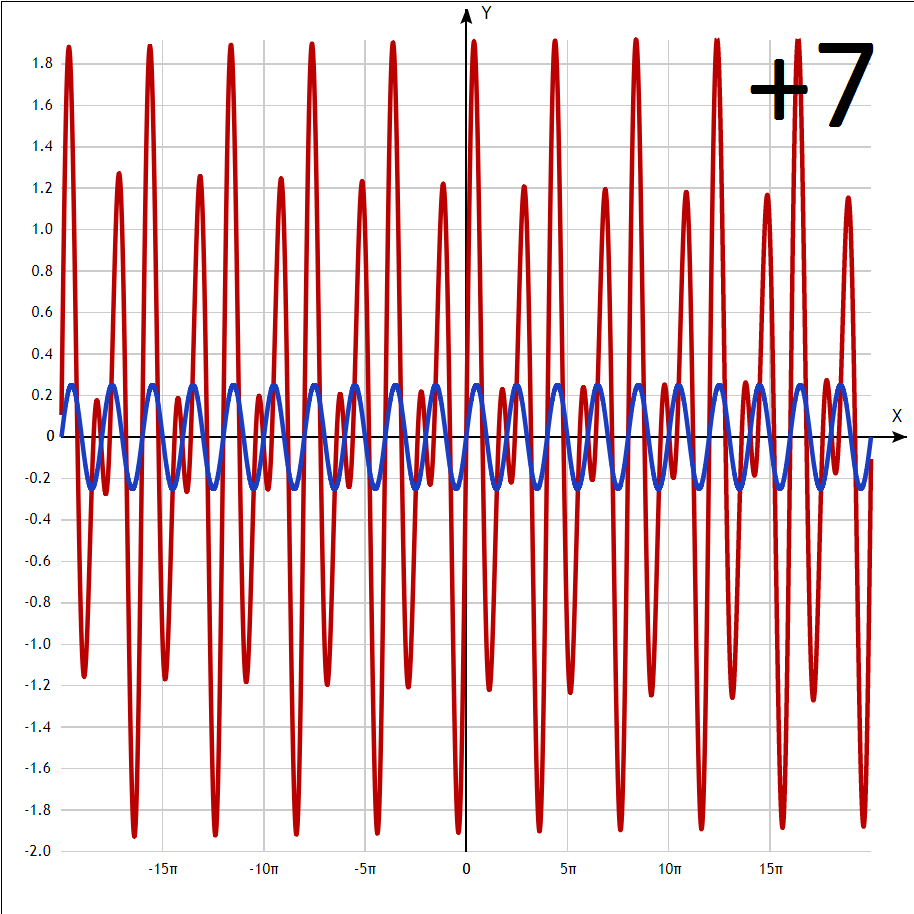
\includegraphics[width=0.45\textwidth]{fig/intervals/i07} \\
        \hline\hline
    \end{tabular}
\end{table}

\begin{table}[!ht]
    \caption{Диссонанс в графике функции \eqref{eq:harmony:interval:sin}}
    \label{t:harmony:interval:disso-6}
    \centering
    \begin{tabular}{c}
        \hline\hline
        6 полутонов, $n=6$ \\
        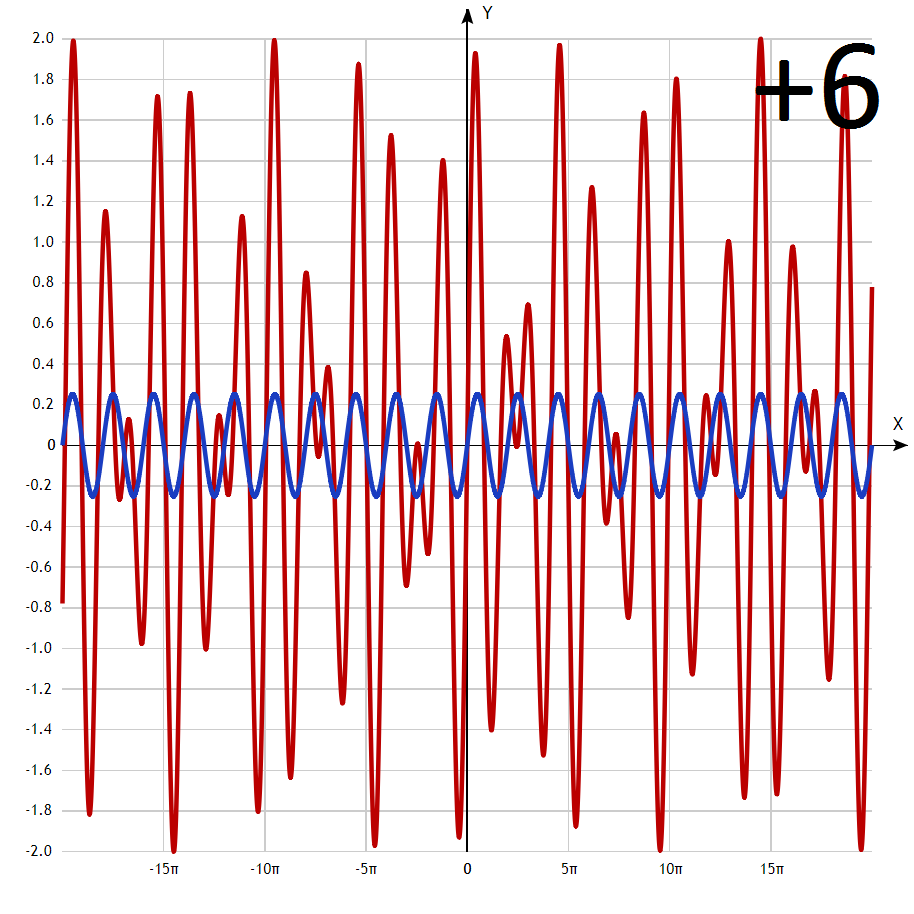
\includegraphics[width=0.45\textwidth]{fig/intervals/i06} \\
        увеличенная кварта,\\
        она же --- уменьшенная квинта,\\
        он же --- тритон\\
        \hline\hline
    \end{tabular}
\end{table}

Звуки октавы удобно зациклить и изобразить на окружности. На рисунке \ref{fig:harmony:interval:oct-round} изображены ноты октавы и отмечены консонансы и диссонансы от ноты ДО (т.е. C --- ноты обозначены в латинской нотации). Кстати, можно сделать удобный приборчик для определения консонансов и диссонансов, если сделать кружок с нотами подвижным. Но погодите. Если уж делать, то квинто-квартовый круг (см. раздел \ref{ch:harmony:kvinto-kvarto-round}).

\begin{figure}[!ht]
    \centering
    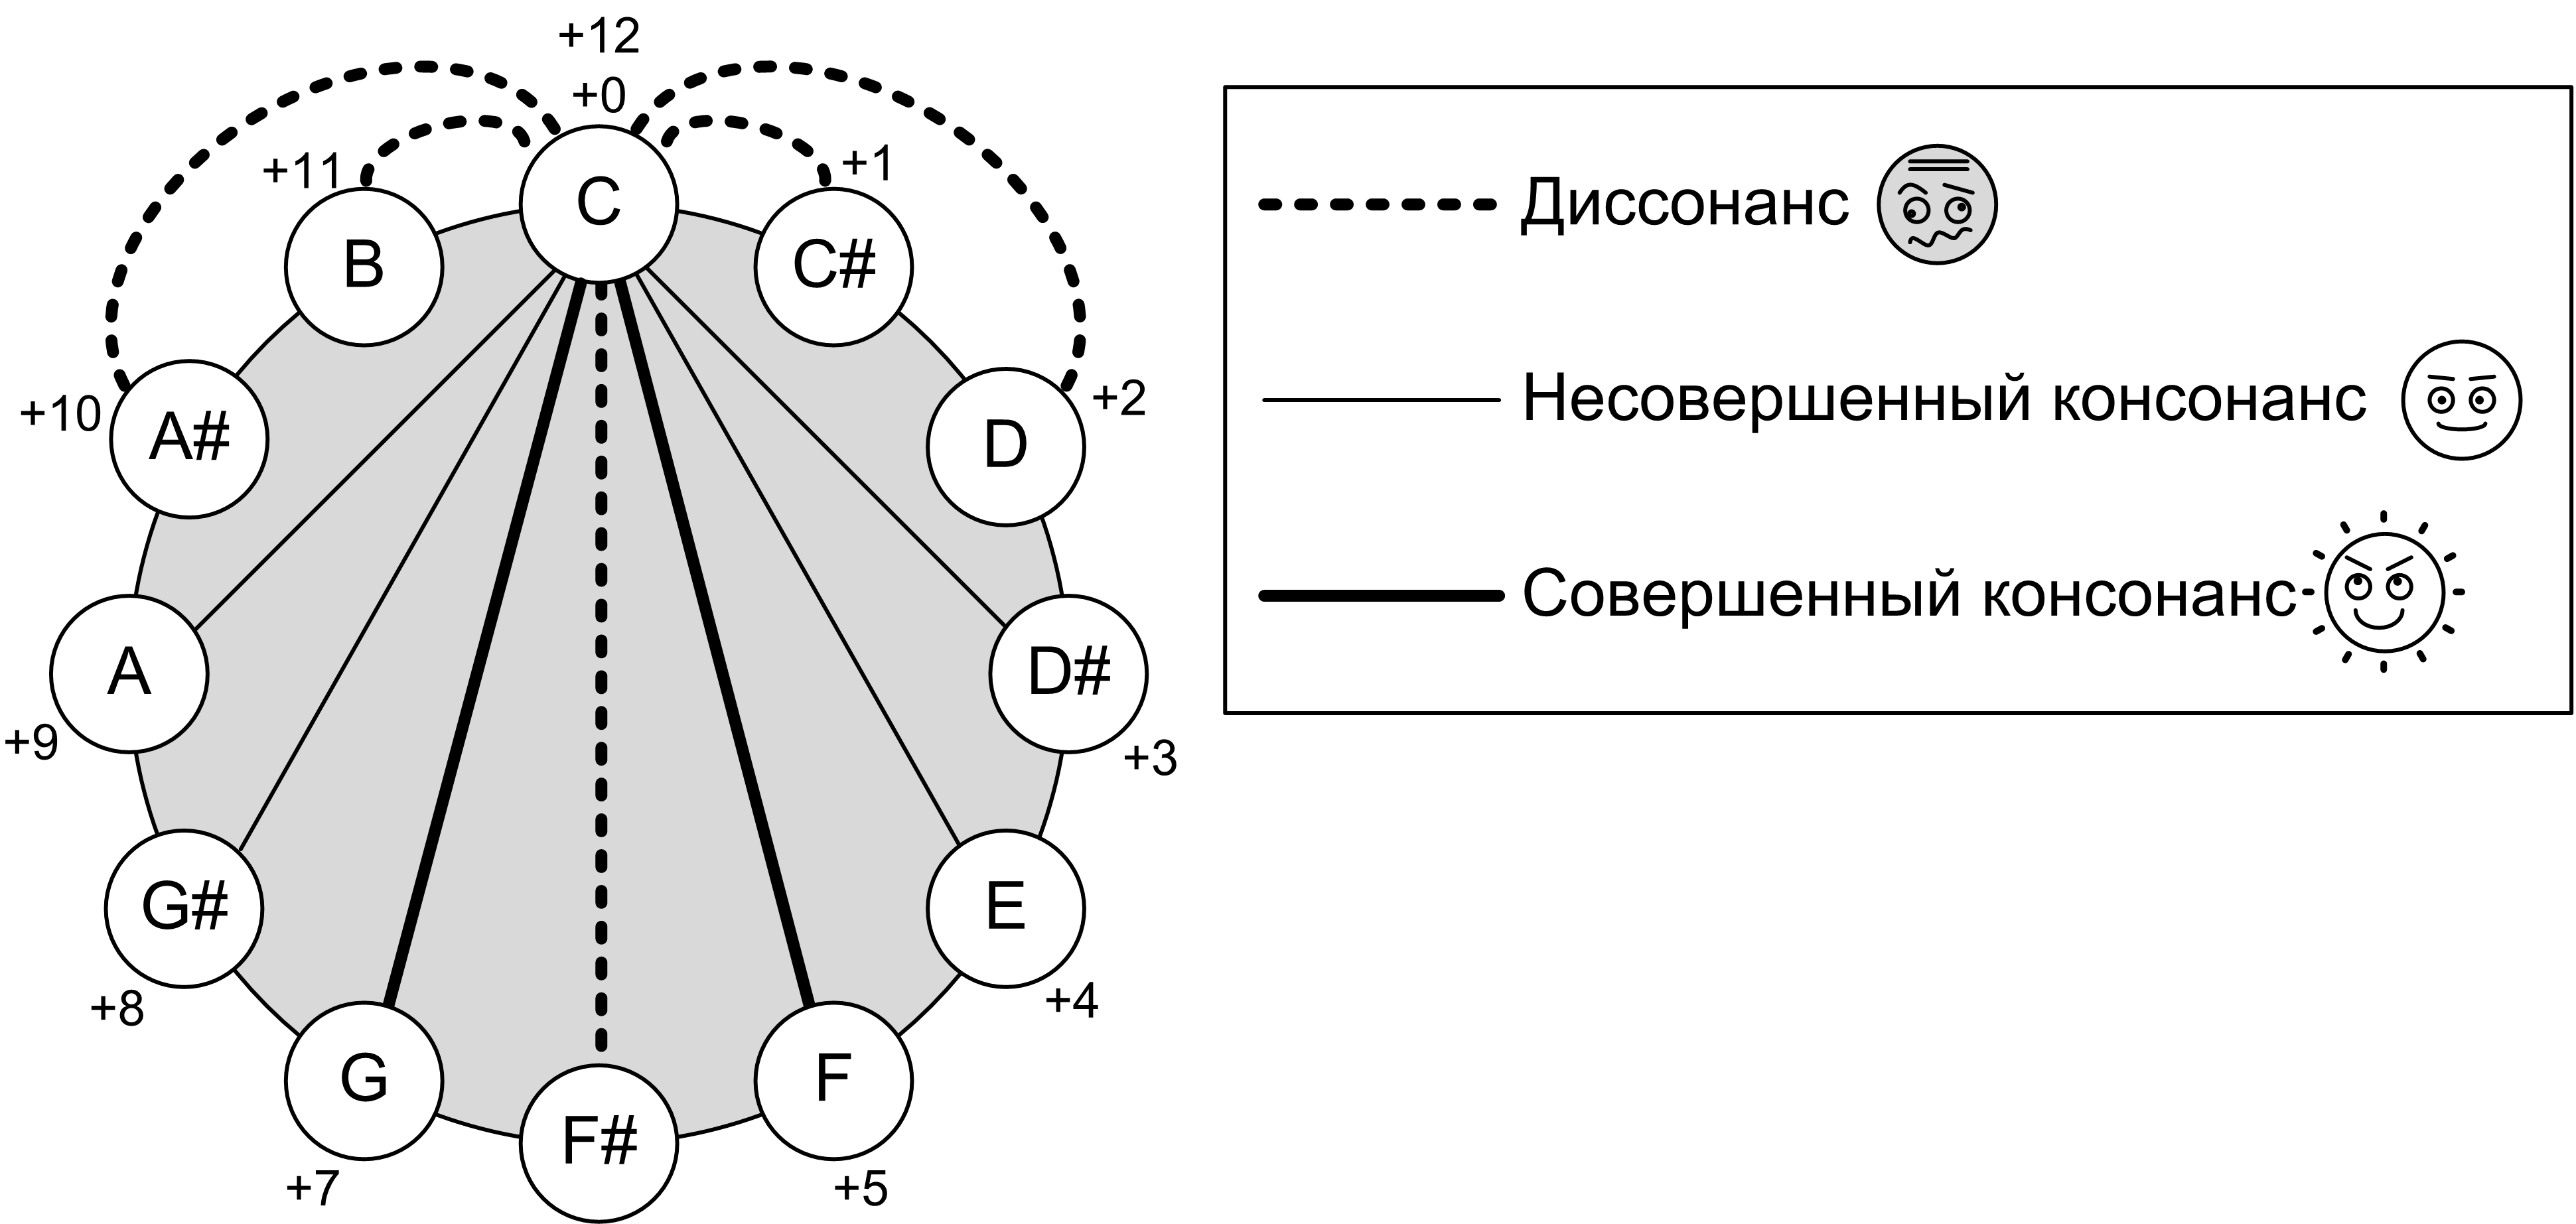
\includegraphics[width=\textwidth]{fig/intervals/octave-round} 
    \caption{Интервалы от ноты ДО}\label{fig:harmony:interval:oct-round}
\end{figure} 

Осталось разобраться какого лешего интервалы называются так странно? Нет никакой видимой связи между названиями интервала и количеством полутонов, его составляющих! Справочник\footnote{Для тех, кому зубрежка покажется проще понимания} по интервалам см. в таблице \ref{t:harmony:interval:names}. Собственно, ответ прост: по историческим причинам название интервала отражало не количество полутонов, а номер ступени мажорного музыкального лада (о ладах см. раздел \ref{ch:harmony:lad}). Так как каждая ступенька мажорного лада состояла из одного или двух полутонов, то определить количество полутонов по названию интервала без достаточного опыта затруднительно, если не представить в уме рисунок \ref{fig:harmony:interval:names}.

\begin{table}[!ht]
    \caption{Интервалы}
    \label{t:harmony:interval:names}
    \centering
    \begin{tabular}{l|l|l|c|l}
        \hline\hline
        Название интервала & Перевод            &               & Количество  & Кратко  \\
                           & на русский         &               & полутонов   &         \\
        \hline\hline
        Прима(prima)       & Первая (ступень)   & Чистая        & 0                 & ч.1 \\
        Секунда(secunda)   & Вторая             & Малая         & 1                 & м.2 \\
                           &                    & Большая       & 2                 & б.2 \\
        Терция(tertia)     & Третья             & Малая         & 3                 & м.3 \\
                           &                    & Большая       & 4                 & б.3 \\
        Кварта(quarta)     & Четвертая          & Чистая        & 5                 & ч.4 \\
                           &                    & Увеличенная   & 6                 & ув.4\\
        Квинта(quinta)     & Пятая              & Уменьшенная   & 6                 & ум.5\\
                           &                    & Чистая        & 7                 & ч.5 \\
        Секста(sexta)      & Шестая             & Малая         & 8                 & м.6 \\
                           &                    & Большая       & 9                 & б.6 \\
        Септима(septima)   & Седьмая            & Малая         & 10                & м.7 \\
                           &                    & Большая       & 11                & б.7 \\
        Октава(octava)     & Восьмая            & Чистая        & 12                & ч.8 \\
        \hline\hline
        Нона(nona)         & Девятая            & Малая         & 13                & м.9  \\
                           &                    & Большая       & 14                & б.9  \\
        Децима(decima)     & Десятая            & Малая         & 15                & м.10 \\
                           &                    & Большая       & 16                & б.10 \\
        Ундецима           & Одиннадцатая       & Чистая        & 17                & ч.11 \\
                           &                    & Увеличенная   & 18                & ув.11\\
        Дуодецима          & Двенадцатая        & Уменьшенная   & 18                & ум.12\\
                           &                    & Чистая        & 19                & ч.12 \\
        Терцдецима         & Тринадцатая        & Малая         & 20                & м.13 \\
                           &                    & Большая       & 21                & б.13 \\
        Квартдецима        & Четырнадцатая      & Малая         & 22                & м.14 \\
                           &                    & Большая       & 23                & б.14 \\
        Квинтдецима        & Пятнадцатая        & Чистая        & 24                & ч.15 \\
        \hline\hline
    \end{tabular}
\end{table}

\begin{figure}[!ht]
    \centering
    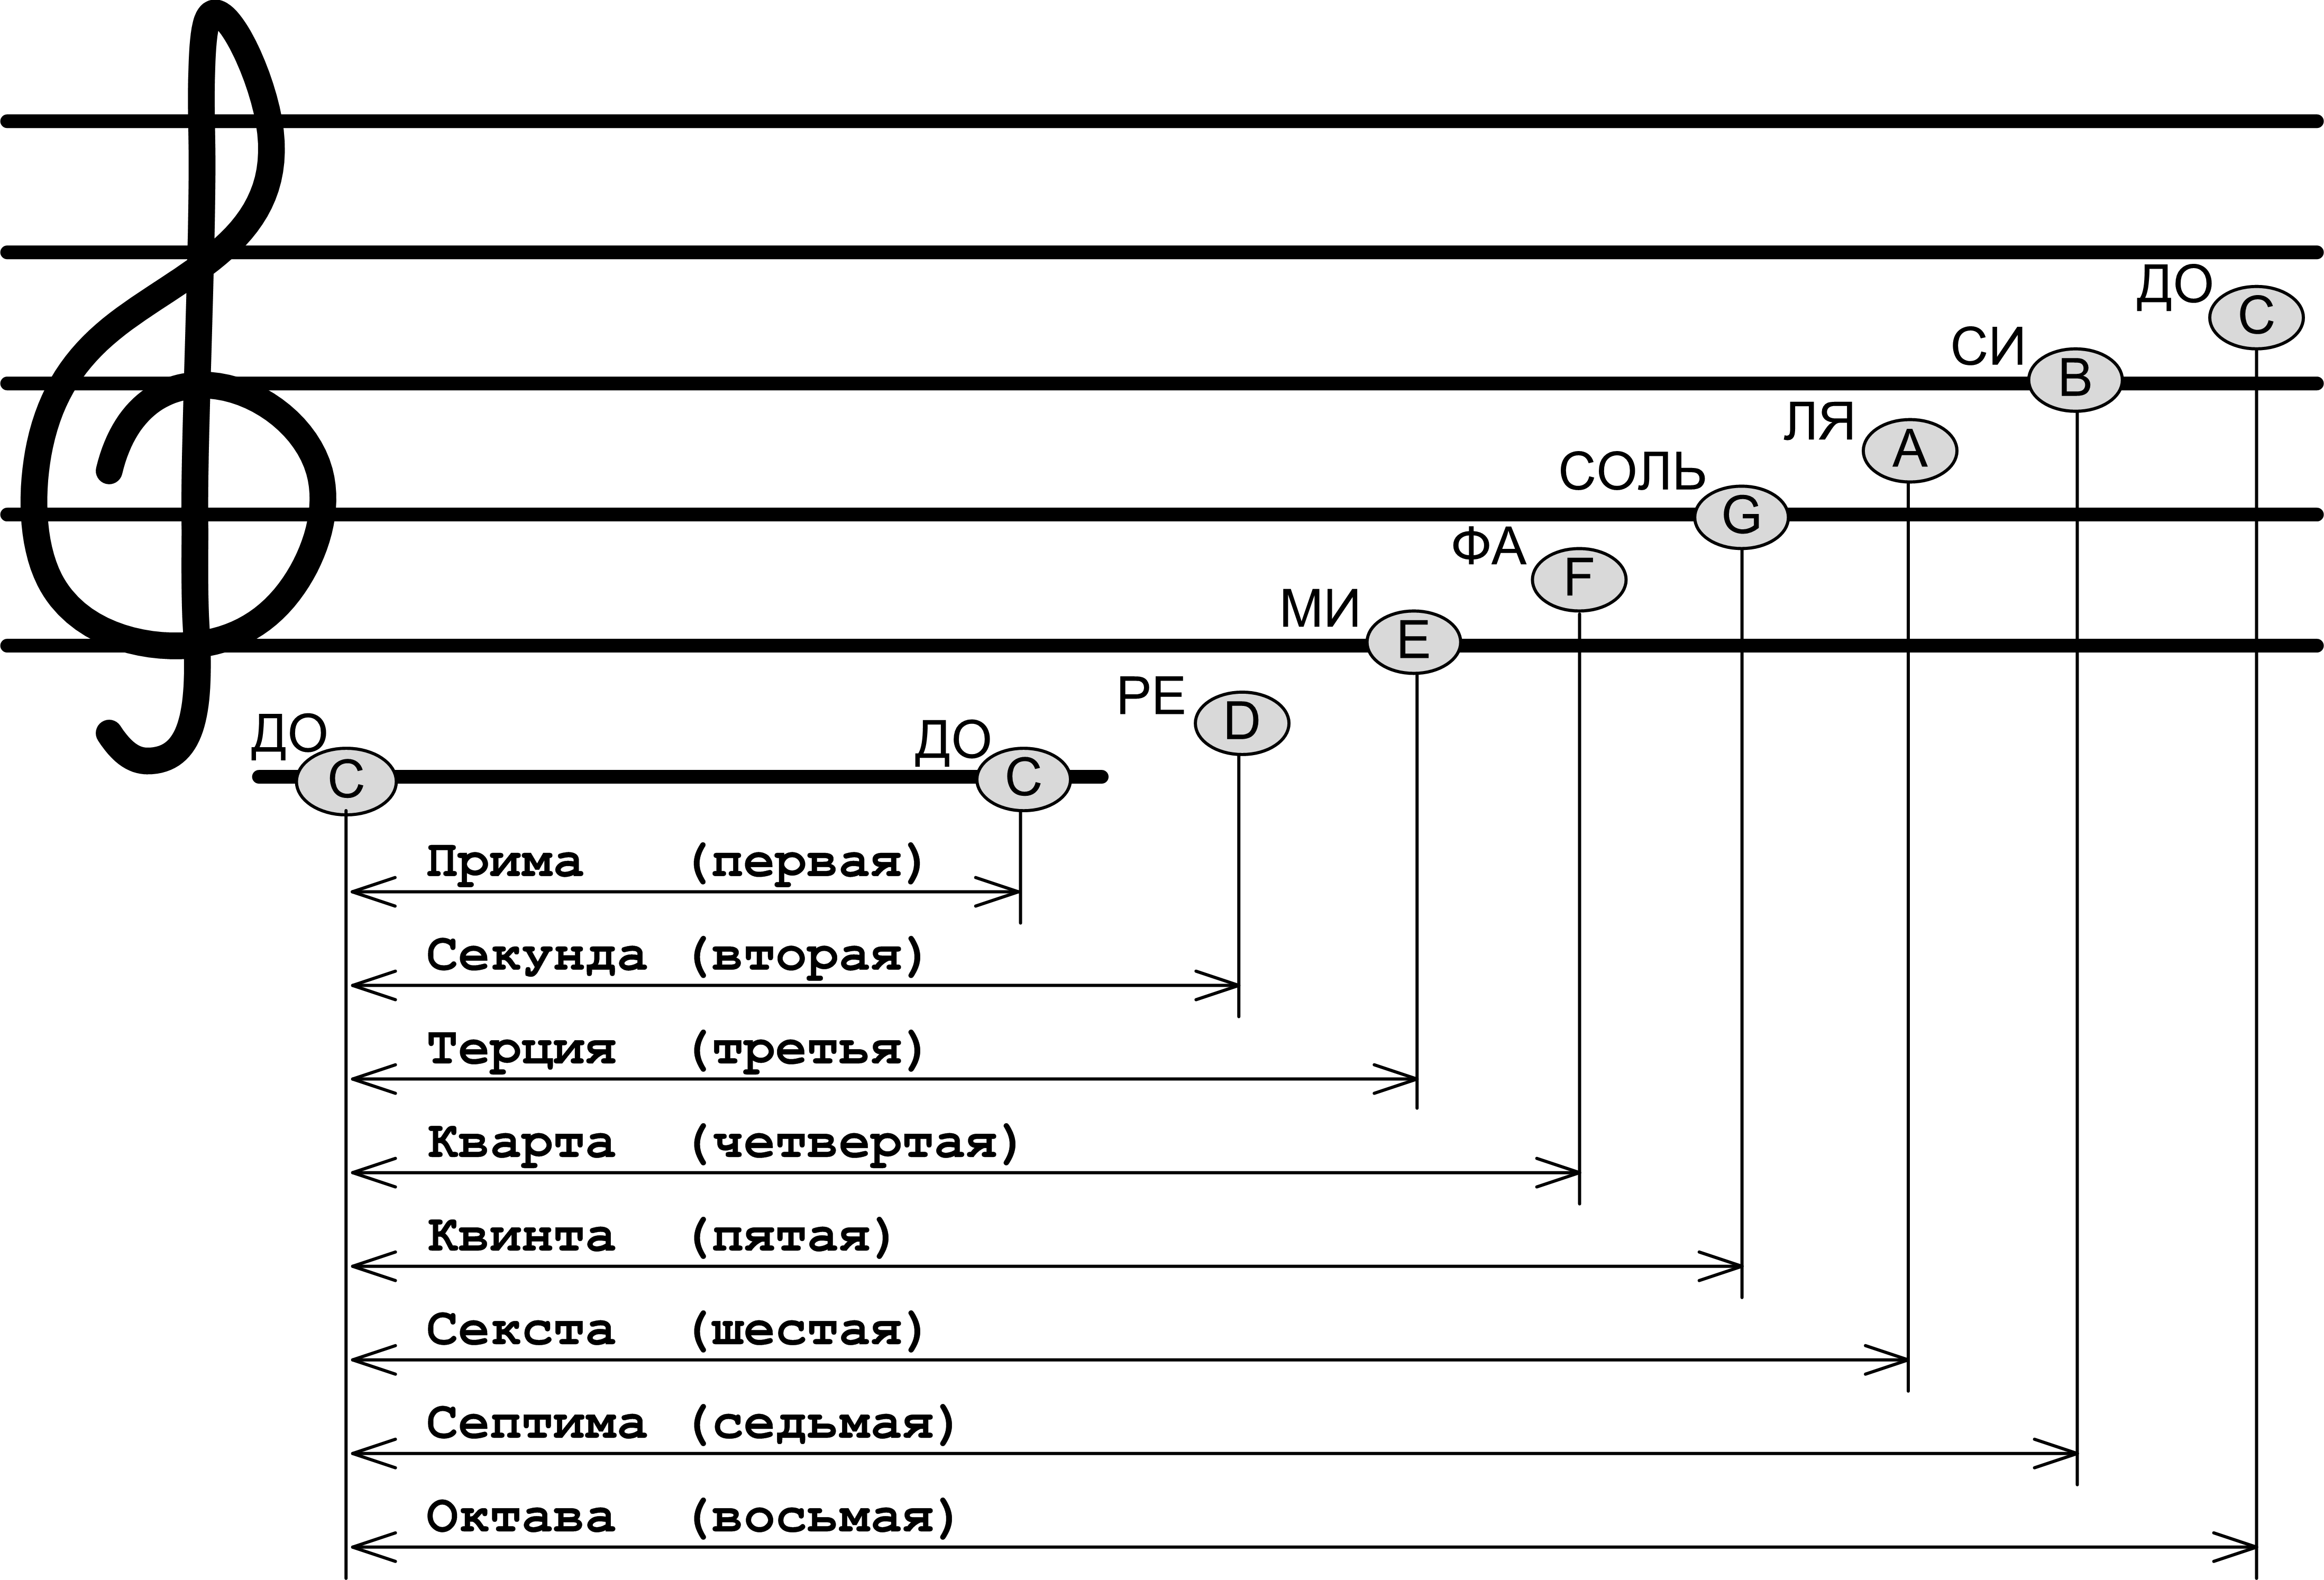
\includegraphics{fig/intervals/interval-names} 
    \caption{Исторически имена интервалов --- это имена ступеней мажорного лада}\label{fig:harmony:interval:names}
\end{figure} 

Тогда все становится относительно просто. Например, терция, это расстояние от ноты ДО (первая ступень мажорного лада) до ноты МИ (третья ступень). Считаем ДО-РЕ --- 2 полутона, РЕ-МИ --- 2-а полутона. Получилось 4-е полутона. Только вот вспоминается, что терция бывает <<большая>> и <<малая>>. При таком подходе мы всегда будем получать значение для <<большого>> и <<чистого>> интервалов. Для <<малого>> или <<уменьшенного>> интервалов нужно уменьшить получившееся число на 1, а для <<увеличенного>> --- увеличить на 1. Значит: большая терция --- 4 полутона, малая --- 3.

Закрепим. Например, квинта: расстояние ДО-СОЛЬ --- 7 полутонов. Уменьшенная квинта --- 6 полутонов, чистая --- 7.
